\newpage
\section{Experimental setup and procedure}
    \subsection{Experimental setup}
        The diode laser setup consists of the diode laser itself
        with a permanently fixed collimator lens and a diffraction grating
        to complete the so-called "Littrow-setup".
        The horizontal orientation of the laser light and with it the length of the external cavity
        and the resulting wavelength can be adjusted by twisting a knob attached to the side.
        Furthermore there are different optical instruments available,
        like lenses, filters, a 50/50 beamsplitter,
        a detector card to make the infra-red light visible,
        a CCD camera and two photodiodes.
        The latter ones are connected to an oscilloscope and are being controlled
        via a power supply, where the current responsible for the laser intensity
        can be varied as well.
        \subsection{Determination of the threshold current}
            As a first step the laser threshold current $I_{Th}$ is determined.
            $I_{Th}$ is given as the minimal current needed for the diode laser
            to leave the LED-area and for lasing to take place.
            Therefore the detector card is placed in the beam path
            and the current is slowly raised at the power supply.
            The change to the visible pattern is observed with the CCD camera,
            as seen in figure \ref{fig:Aufbau1}.
            \begin{figure}[h]
                \centering
                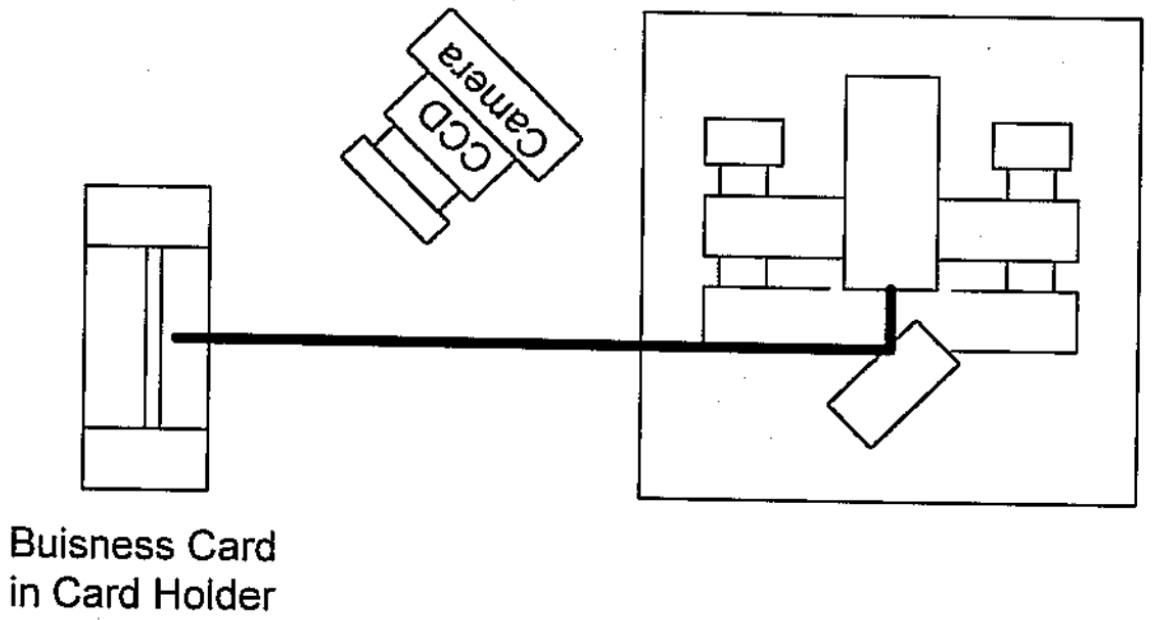
\includegraphics[width = 0.7\textwidth]{pictures/Aufbau1.png}
                \caption{Setup for the determination of the threshold current. Taken from \cite{tu_dortmund_versuchsanleitung_2022-1}.}
                \label{fig:Aufbau1}
            \end{figure}
        \subsection{Recording of the rubidium fluorescence}
            Next, the laser light is directed onto a rubidium cell.
            The current is set to a value $I\gg I_{Th}$ and
            the CCD camera is placed orthogonal to the beam orientation
            with the possibility to record the interior of the cell.
            The described setup is represented in figure \ref{fig:Aufbau2}.
            The angle of the grating is adjusted precisely by a build-in piezo crystal,
            which allows to make the rubidium emission line permanently visible.
            \begin{figure}[h]
                \centering
                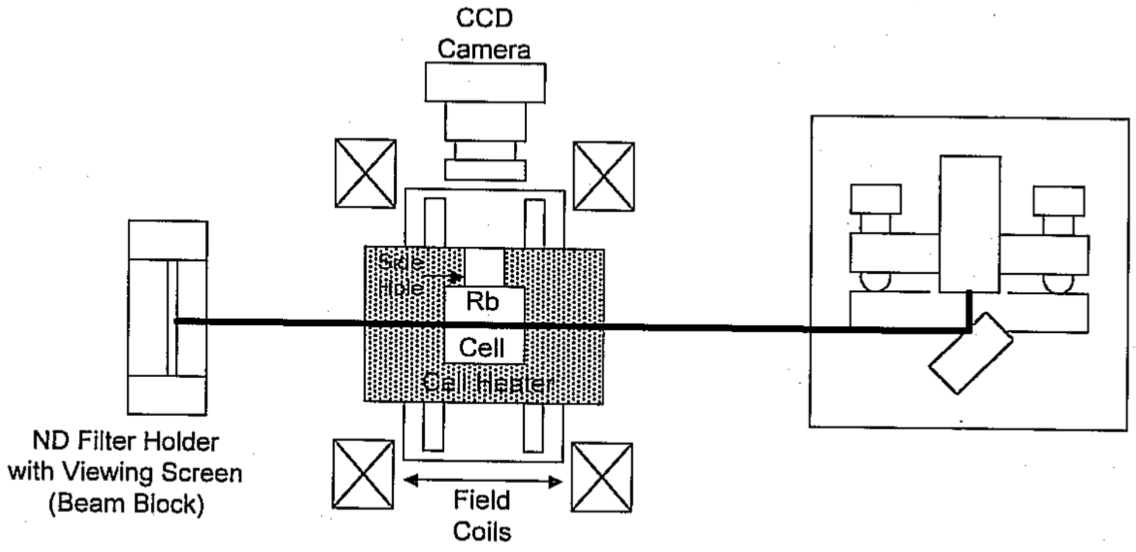
\includegraphics[width = 0.7\textwidth]{pictures/Aufbau2.png}
                \caption{Setup for the recording of the rubidium fluorescence. Taken from \cite{tu_dortmund_versuchsanleitung_2022-1}.}
                \label{fig:Aufbau2}
            \end{figure}
        \subsection{Measuring the absorption spectrum of rubidium}
            Lastly, a beamsplitter is positioned between the laser source and the rubidium cell.
            At the end of each outgoing beam path a photodiode is placed (see figure \ref{fig:Aufbau3}).
            Both of them are connected to the oscilloscope,
            where their signals are subtracted from one another,
            so that the background is filtered out and
            just the voltage change due to the rubidium absorption is shown.
            The current and wavelength are adjusted by the piezo and control-knob that
            all 4 absoption peaks are visible within one mode on the oscilloscope with no mode-hops in between.
            \begin{figure}[h]
                \centering
                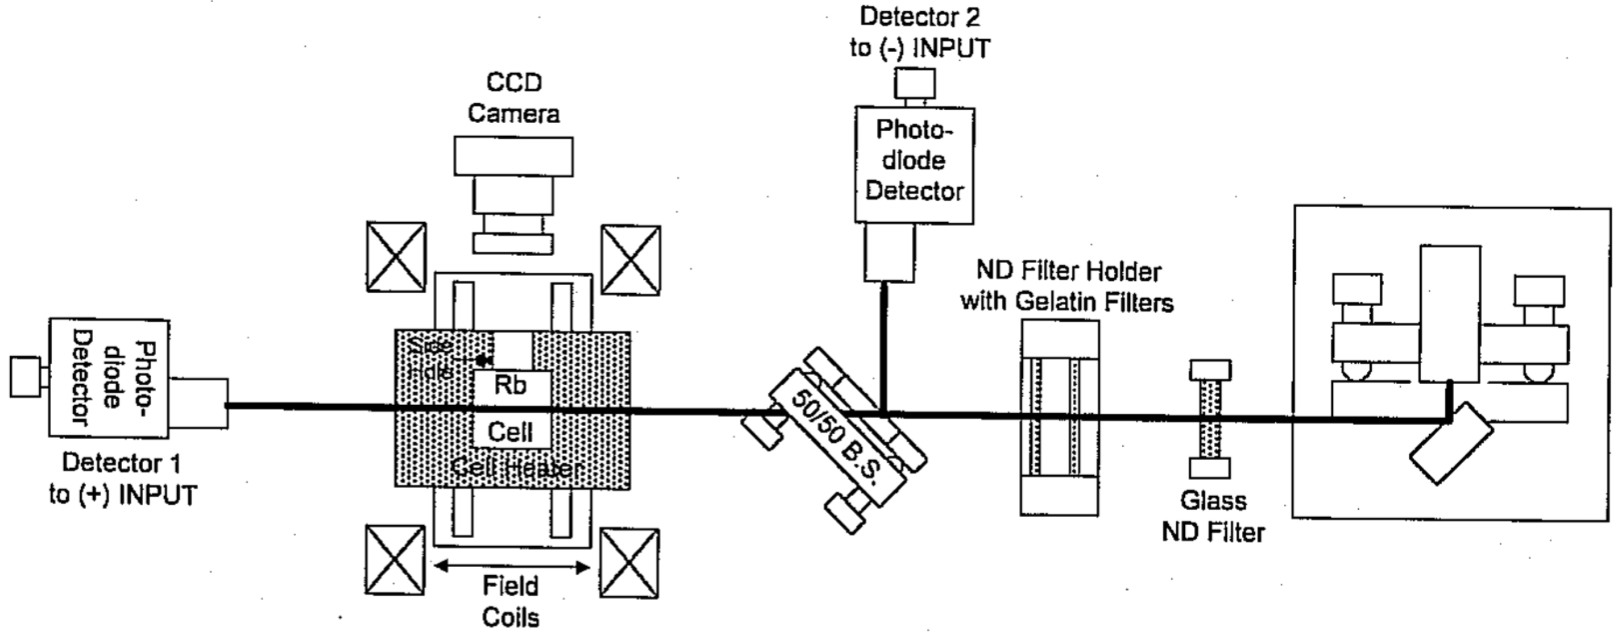
\includegraphics[width = 0.7\textwidth]{pictures/Aufbau3.png}
                \caption{Setup for measuring the absorption spectrum of rubidium. Taken from \cite{tu_dortmund_versuchsanleitung_2022-1}.}
                \label{fig:Aufbau3}
            \end{figure}
